\documentclass{beamer}
\usepackage{mathrsfs}  
\usepackage{xcolor}
\usepackage{setspace}
\usepackage{comment}
\usepackage{lmodern}
\usepackage[utf8x]{inputenc}
\usepackage[T1]{fontenc}

% config du thgeme metropolis
\usetheme[progressbar=frametitle,block=fill, titleformat=smallcaps,sectionpage=progressbar,]{metropolis}



\title{Statistiques, Probabilités, Analyse Spatiale}
\subtitle{Présentation du Module}
\date{2021-2022}
\author{Paul Chapron \textsuperscript{1} \& Yann Ménéroux \textsuperscript{1} \& Juste Raimbault }
\institute{ \textsuperscript{1}IGN-ENSG-UGE}



%definition de la couleur du texte dans la balise \alert{}
\definecolor{vertIGN}{HTML}{96C31E} % vert IGN %vrai valeur #97BE0D
\setbeamercolor{alerted text}{fg=vertIGN}

\definecolor{grisIGN}{HTML}{22292F} % Gris IGN tiré vers le noir 
\setbeamercolor{background canvas}{bg=grisIGN}




% code pour placer le log ENSG dans le bandeau de titre 
\makeatletter
\setbeamertemplate{frametitle}{%
  \nointerlineskip%
  \begin{beamercolorbox}[%
      wd=\paperwidth,%
      sep=0pt,%
      leftskip=\metropolis@frametitle@padding,%
      rightskip=\metropolis@frametitle@padding,%
    ]{frametitle}%
  \metropolis@frametitlestrut@start%
  \insertframetitle%
  \nolinebreak%
  \metropolis@frametitlestrut@end%
  \hfill
  \raisebox{-0.6ex}{
\includegraphics[height=4ex,keepaspectratio]{img/logoENSG_small.jpg}}
  \end{beamercolorbox}%
}
\makeatother




% logo ENSG première page 
\titlegraphic{\vspace{4cm}\flushright
\includegraphics[width=2cm,height=2cm]{img/logoENSG_big.png}} 



\begin{document}
\metroset{background=dark} % change background theme according to manual
\maketitle	

\section{Introduction} 



\begin{frame}
\frametitle{Citations en vrac}

\begin{tiny}


\hfill «If you torture data long enough, it will confess» \\
\hfill Ronald Coase\\
\vfill
\hfill «It is a capital mistake to theorize before one has data.»\\
\hfill Sherlock Holmes\\
\vfill
\hfill «All models are wrong, but some are useful.»\\
\hfill  George Box\\
\vfill
\hfill «Data scientist (noun): Person who is better at statistics than any software engineer and better at software engineering than any statistician.»\\
\hfill Josh Wills\\
\vfill
\hfill «There are lies, damned lies and statistics» \\
\hfill Mark Twain\\ 
\vfill

\hfill «Les statistiques sont une forme d'accomplissement de désir, tout comme les rêves.» \\
\hfill Jean Baudrillard\\
\vfill



\hfill «Ce qui est simple est faux, ce qui est compliqué est inutile.» \\
\hfill Paul Valéry\\
\vfill


\hfill «La statistique est la première des sciences inexactes.»\\
\hfill  Édouard et Jules de Goncourt



\end{tiny}


\end{frame}





\begin{frame}
\frametitle{Survol des trois thématiques}
\begin{itemize}
\item \alert{Statistique} : Démarche scientifique visant à acquérir des connaissances sur l'état d'un objet difficilement perceptible sur le plan cognitif : 
\begin{itemize}
\item objet \alert{massif} (population, big data...) : résumer, synthétiser, visualiser, échantillonner, compresser...
\item objet \alert{incertain} (observations bruitées) : moyenner, borner, encadrer, compenser... \newline \pause
\end{itemize}

En général, la statistique sert à  \alert{décrire} des états présents ou passés.


\end{itemize}
\end{frame}


\begin{frame}
\frametitle{Survol des trois thématiques}

\begin{itemize}
\item \alert{Probabilités} : théorie mathématique traitant de l'aléatoire, sans justification a priori (même si généralement fondée sur des besoins pratiques) et opérant dans un cadre contrôlé (information parfaite).
\newline \pause
\end{itemize}
En général, les probabilités servent à  \alert{prédire} des états futurs.
\end{frame}




\begin{frame}
\frametitle{Survol des trois thématiques}
\begin{itemize}
\item \alert{Analyse Spatiale} : Étude de la répartition et de l’organisation d’objets localisés pour «déceler en quoi la localisation apporte un élément utile à la connaissances des objets étudiés et peut en expliquer les caractéristiques» \[Pumain, Saint-Julien 1997\]
\newline \pause
\end{itemize}


Nous couvrirons principalement l'analyse spatiale \alert{statistique} qui utilisent de nouvelles variables : les coordonnées des objets et les distances  qui les séparent.
\end{frame}






\begin{frame}
\frametitle{Programme du module}


\centering
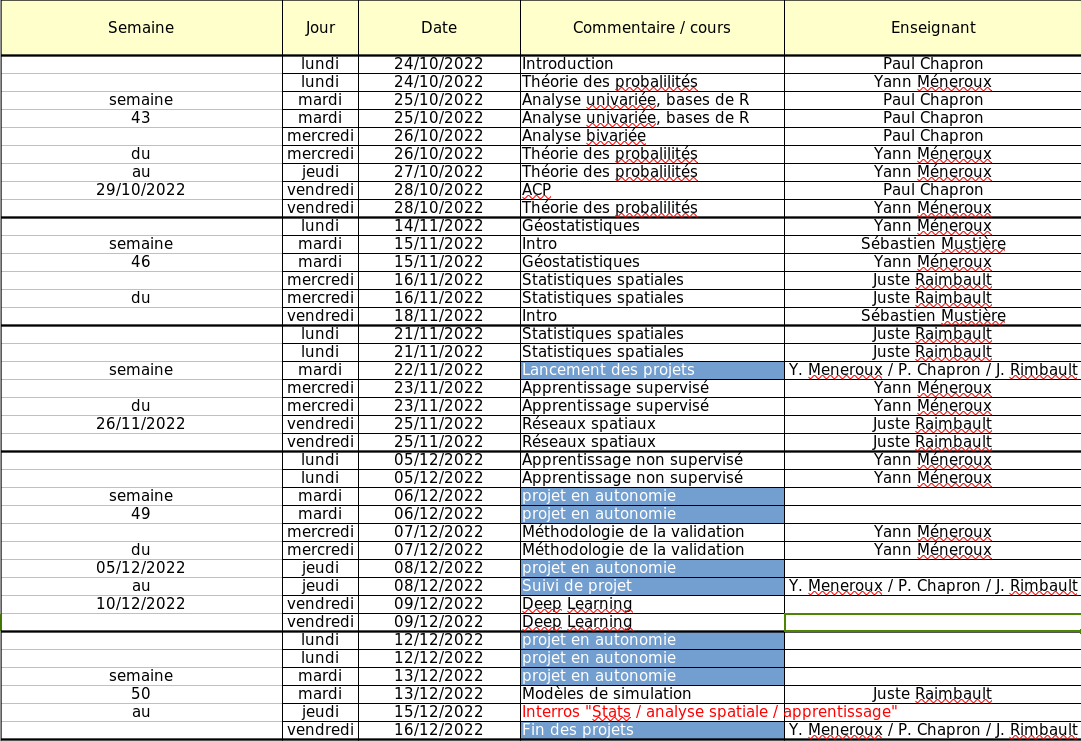
\includegraphics[width=\textwidth,keepaspectratio]{img/agenda2022.png}

\end{frame}


\setbeamercolor{background canvas}{bg=white}



\begin{frame}
\frametitle{Naissance au XVIIe ?}

\begin{center}

      \includegraphics<1>[scale=0.40, trim = 1.3cm 1.3cm 1.3cm 1.3cm, clip]{img/platee/platee03.pdf}
      \includegraphics<2>[scale=0.40, trim = 1.3cm 1.3cm 1.3cm 1.3cm, clip]{img/platee/platee03.pdf}
      \includegraphics<3>[scale=0.40, trim = 1.3cm 1.3cm 1.3cm 1.3cm, clip]{img/platee/platee04.pdf}
      \includegraphics<4>[scale=0.40, trim = 1.3cm 1.3cm 1.3cm 1.3cm, clip]{img/platee/platee05.pdf}
      \includegraphics<5>[scale=0.40, trim = 1.3cm 1.3cm 1.3cm 1.3cm, clip]{img/platee/platee06.pdf}
      \includegraphics<6>[scale=0.40, trim = 1.3cm 1.3cm 1.3cm 1.3cm, clip]{img/platee/platee07.pdf}
      \includegraphics<7>[scale=0.40, trim = 1.3cm 1.3cm 1.3cm 1.3cm, clip]{img/platee/platee08.pdf}
      \includegraphics<8>[scale=0.40, trim = 1.3cm 1.3cm 1.3cm 1.3cm, clip]{img/platee/platee09.pdf}
      \includegraphics<9>[scale=0.40, trim = 1.3cm 1.3cm 1.3cm 1.3cm, clip]{img/platee/platee10.pdf}
      \includegraphics<10>[scale=0.40, trim = 1.3cm 1.3cm 1.3cm 1.3cm, clip]{img/platee/platee11.pdf}
      \includegraphics<11>[scale=0.40, trim = 1.3cm 1.3cm 1.3cm 1.3cm, clip]{img/platee/platee12.pdf}
\end{center} 
\end{frame}


\setbeamercolor{background canvas}{bg=grisIGN}




\begin{frame}
\frametitle{Naissance des probabilités}


\textbf{Correspondance de Pascal et Fermat (1654) :} \textit{Deux joueurs déposent chacun une mise $m$ pour jouer une partie en 3 manches, mais décident de se quitter après deux victoires de l'un et une victoire de l'autre. Comment devraient-ils se répartir la mise ?}

\begin{itemize}
\item probabilisme (XVI\textsuperscript{ème} siècle)
\item Pas d'utilisation en dehors des jeux
\item Leibniz : outil de connaissance et de raisonnement sur le réel. La Statistique devient un instrument scientifique (1677)
\item Paradoxe de Saint-Petersbourg (1713)
\item  Bayes : théorie des causes (1763)
\item Fin XVIII\textsuperscript{ème} : Arithmétique politique (démographie, tables de mortalité, etc)
\end{itemize}
\end{frame}

\end{document}